\subsubsection{$\Wmn$ Event Selection}
\label{sec:WmnSel}

% $\Wmn$ events are characterized by a high-$\Pt$, isolated muon,
% together with a significant amount of missing $\Et$, due to the
% presence of a neutrino in the final-state, that escapes undetected.

The first step in the $\Wmn$ candidate selection is to
reject those events having two global muons satisfying: $\Pt(\mu_1) >
20~\GeV$ and $\Pt(\mu_2) > 10~\GeV$, where $\Pt(\mu_1)$ is the
highest muon $\Pt$ and $ \Pt(\mu_2)$ is the second highest muon $\Pt$
in the event, in order to minimize the contamination from DY
events.

Events with a good quality muon, as described in Section~\ref{sec:muonid},
in the fiducial volume $|\eta|<2.1$, and with a transverse momentum
higher than $25~\GeV$ are kept.
Relative combined isolation variable (see Section~\ref{sec:isolation}) is used to evaluate the level of activity around the
muon. Isolation distribution of the experimental data, together with the simulation expectations, is shown in
Fig.~\ref{figure:Wmunu_iso}. The muon is considered to be isolated if $\IRelComb < 0.1$.
Events with $\IRelComb > 0.2$ are mainly coming from QCD background, and are be used as 
control sample (see Section~\ref{sec:WQCDbkg}).

\begin{figure}[htb] {\centering
    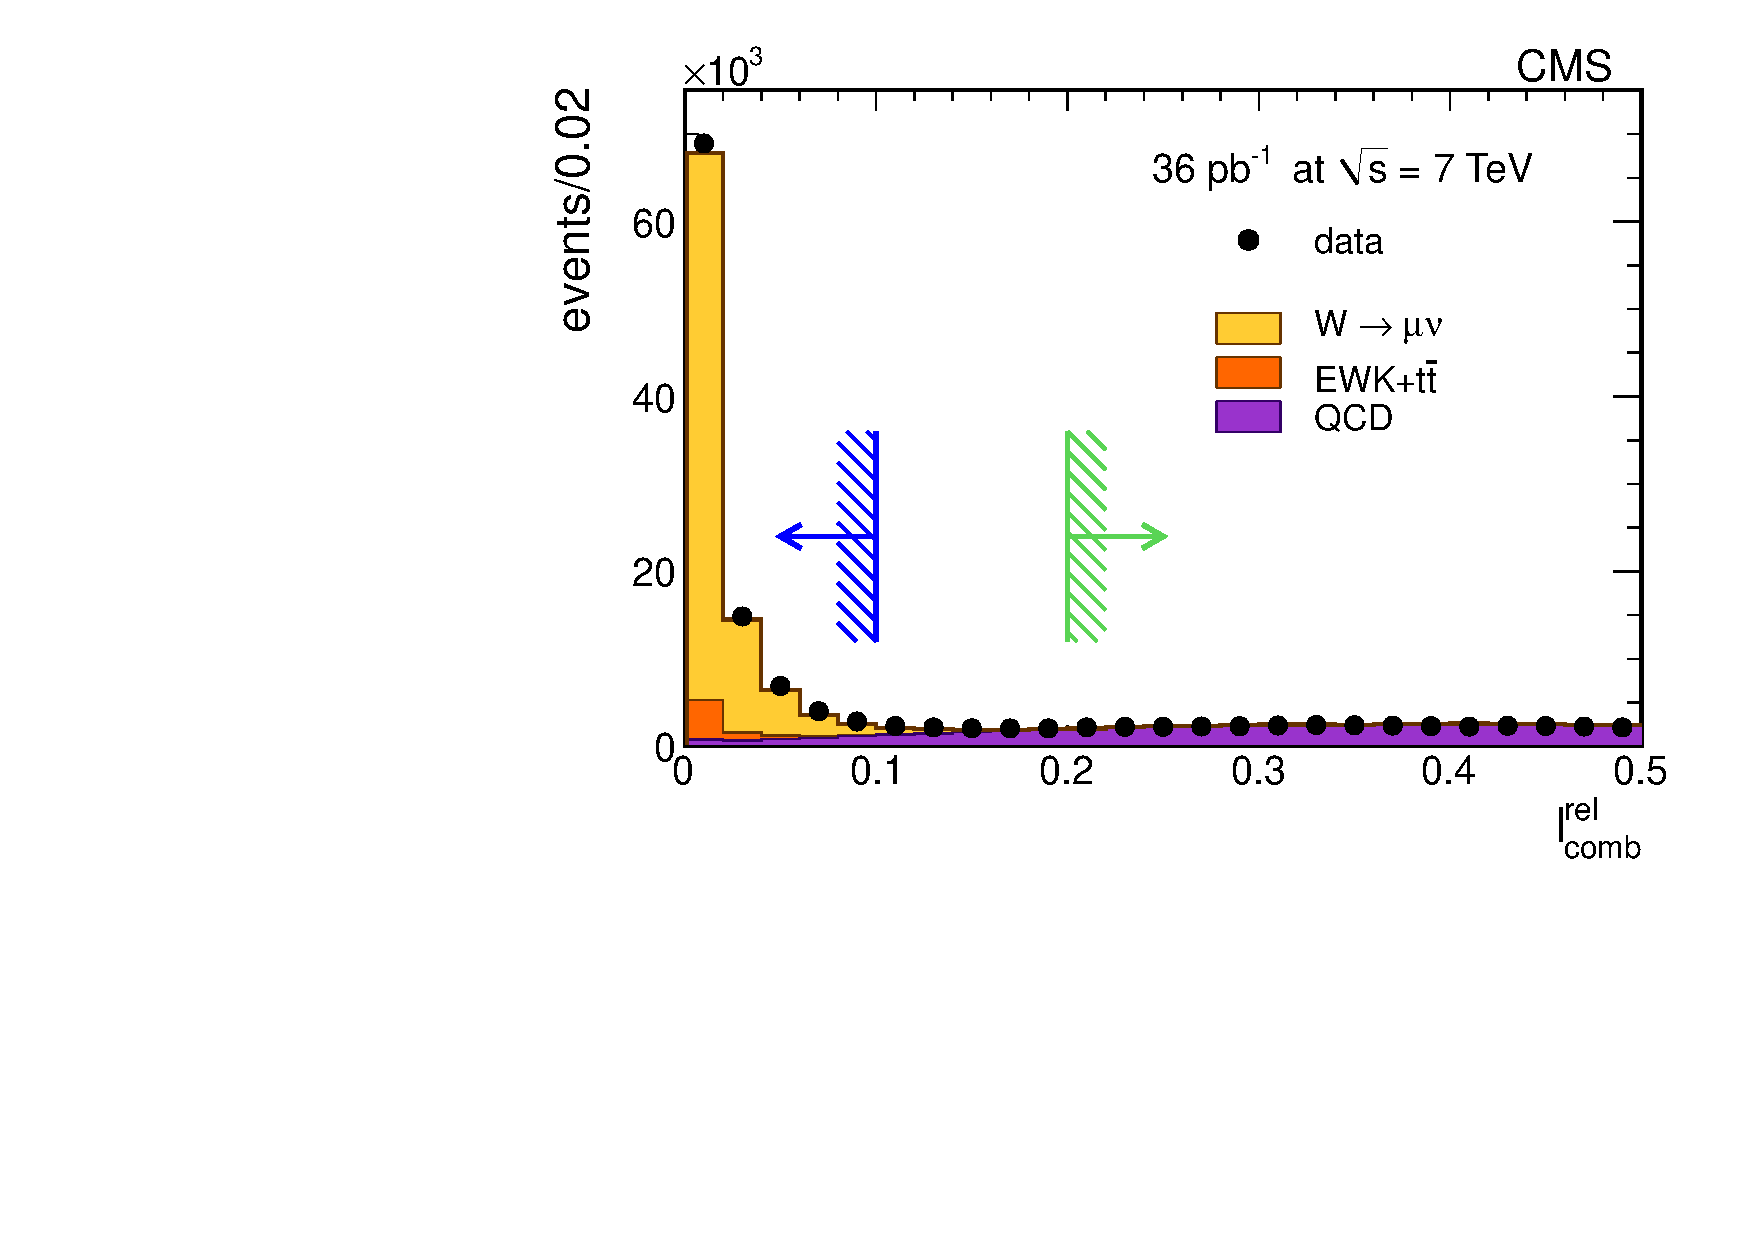
\includegraphics[width=8cm]{figs/Wmunu_isolation.pdf}
    \caption{Isolation distribution of $\Wmn$ candidates with a good quality muon of $\Pt>25~\GeV$ in the fiducial region $|\eta|<2.1$.
Dots represent the data and the solid histograms the contribution from the different SM processes.
The superimposed arrows represent the signal selection requirement (red
arrow, $\IRelComb<0.1$) and selection of the QCD-enriched
control sample (green arrow, $\IRelComb>0.2$).
}
    \label{figure:Wmunu_iso}}
\end{figure}


% The breakdown of the data reduction at the different stages of the
% selection is summarized in Table~\ref{table:Wmunu_selection} both for
% the total sample of muon events, and split by the muon charge.
% %%%%%%%%
% \begin{table}[!ht] 
% \begin{center}
% \begin{tabular}{|c||c|c|c|} \hline
% {Event Sample}                           & Events with $\mu^\pm$ &  Events with $\mu^+$ & Events with $\mu^-$ \\ \hline \hline
% {Candidates}                             &         6395420       &      1812890        &      1677349      \\
% {Triggered}                              &         3174720       &      1644727        &      1529995      \\
% {DY Rejection}                           &         3133420       &       1623994       &      1509425      \\
% {Muon ID}                                &         2618199       &       1346297       &      1271902      \\
% {$|\eta|<2.1$}                           &         2527047       &       1298777       &      1228270      \\
% {$\Pt > 25 \GeV$}                       &          412266       &        222080       &      190186       \\
% $\IRelComb<0.1$                         &          166457       &         97533       &       68924       \\ \hline
% \end{tabular}
% \caption{Data reduction at every step of the selection process.
% Number of events are given for the whole muon data sample, as well as separated by the muon charge.}
% \label{table:Wmunu_selection}
% \end{center}
% \end{table}

After the selection process just described, 166457 events are selected,
97533 of them with a positive charged muon and 68924 with a negative
charged muon.

